
%(BEGIN_QUESTION)
% Copyright 2006, Tony R. Kuphaldt, released under the Creative Commons Attribution License (v 1.0)
% This means you may do almost anything with this work of mine, so long as you give me proper credit

Fortrengerinstrumenter brukes ofte til nivåmåling av væske:

$$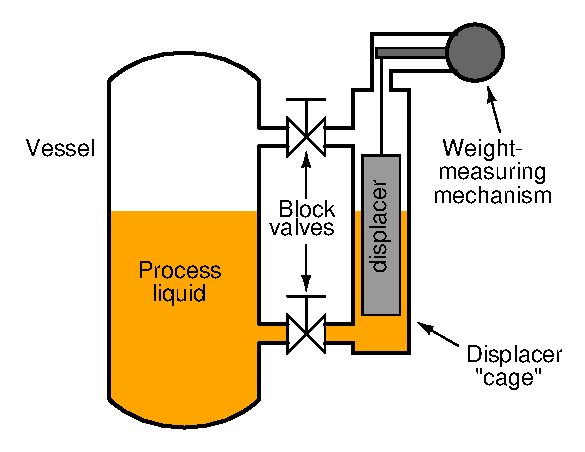
\includegraphics[width=15.5cm]{i00280x01.eps}$$

Hvordan kan et slikt instrument modifiseres for å måle væske-\textit{tetthet} i stedet?

\vskip 20pt \vbox{\hrule \hbox{\strut \vrule{} {\bf Forslag til sokratisk diskusjon} \vrule} \hrule}

\begin{itemize}
\item{} En nyttig problemløsningsmetode her er å studere oppdriftskraft-ligningen og identifisere hvilke fysiske størrelser som er faste og variable i et standard nivåinstrument.  Spør deretter hvilke størrelser som må være faste/variable for å gjøre instrumentet til et \textit{tetthets}-instrument.  Prøv metoden og se om det hjelper.
\end{itemize}

\underbar{file i00280}
%(END_QUESTION)





%(BEGIN_ANSWER)


%(END_ANSWER)





%(BEGIN_NOTES)

For å måle tetthet med et fortrengerinstrument må det konfigureres slik at fortrengeren alltid er \textit{helt} neddykket i væske.  Da vil bare endringer i væsketetthet påvirke fortrengerens vekt.  Jeg lar deg tenke ut konkrete måter å gjøre dette på.

\vskip 10pt

Én måte å sikre full neddykkingen av fortrengeren er denne:

$$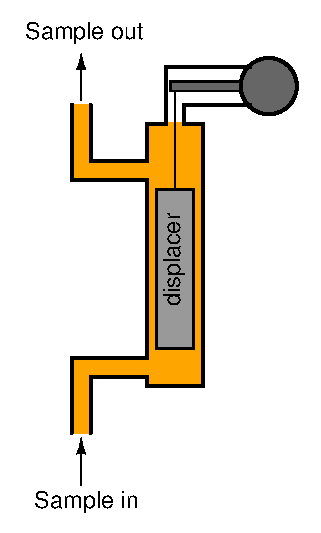
\includegraphics[width=15.5cm]{i00280x02.eps}$$

Selvsagt må prøveflowen være lav nok til at dynamiske krefter på fortrengeren er neglisjerbare.

%INDEX% Measurement, density: displacer (buoyancy)

%(END_NOTES)
